%% Machine Learning with Applications — Elsevier
%% English version v1
%%
%% Compile:
%%   pdflatex main_en_v1
%%   bibtex   main_en_v1
%%   pdflatex main_en_v1
%%   pdflatex main_en_v1

\documentclass[preprint,12pt,authoryear]{elsarticle}

%% ── Packages ──────────────────────────────────────────────────────────────
\usepackage{amsmath,amssymb,amsfonts}
\usepackage{graphicx}
\usepackage{booktabs}
\usepackage{array}
\usepackage{multirow}
\usepackage[table,xcdraw]{xcolor}
\usepackage{hyperref}
\usepackage{cleveref}
\usepackage{lineno}
\usepackage{microtype}
\usepackage{siunitx}
\usepackage{bm}
\usepackage{caption}
\usepackage{subcaption}
\usepackage{enumitem}
\usepackage{algorithm}
\usepackage{algpseudocode}
\algrenewcommand\algorithmicwhile{\textbf{while}}
\algrenewcommand\algorithmicdo{\textbf{do}}
\algrenewcommand\algorithmicend{\textbf{end}}
\algrenewcommand\algorithmicfor{\textbf{for}}
\algrenewcommand\algorithmicif{\textbf{if}}
\algrenewcommand\algorithmicthen{\textbf{then}}
\algrenewcommand\algorithmicelse{\textbf{else}}
\algrenewcommand\algorithmicreturn{\textbf{return}}
\floatname{algorithm}{Algorithm}
\usepackage[utf8]{inputenc}
\usepackage[T1]{fontenc}
\usepackage[english]{babel}

%% Line numbering (required for review)
\linenumbers

\sisetup{separate-uncertainty=true, group-separator={,}, output-decimal-marker={.}}

\hypersetup{
    colorlinks=true,
    linkcolor=blue!70!black,
    citecolor=blue!60!black,
    urlcolor=blue!60!black
}

%% ── Macros ────────────────────────────────────────────────────────────────
\newcommand{\CR}[1]{CR_{2,\text{#1}}}
\newcommand{\RMSE}{\mathrm{RMSE_{CV}}}       % cross-validation
\newcommand{\Rsq}{R^{2}_{\mathrm{CV}}}
\newcommand{\nd}{N_{\mathrm{d}}}
\newcommand{\np}{n_{\mathrm{p}}}              % number of stories
\newcommand{\etad}{\eta}
\newcommand{\Mf}{M_{\!f}}
\newcommand{\ha}{h_a}
\newcommand{\KM}{\,\si{kN{\cdot}m}}

\journal{Machine Learning with Applications}

\begin{document}

\begin{frontmatter}

\title{Machine Learning-Based Optimization of Rotational Friction Dampers in
       Steel Moment-Resisting Frames under Seismic Excitation}

\author[uaq]{E.~Ponce}
\author[i2m]{H.~Yañez-Godoy\corref{cor1}}
\cortext[cor1]{Corresponding author.}
\ead{humberto.yanez-godoy@u-bordeaux.fr}

\address[uaq]{Universidad Autónoma de Querétaro, Faculty of Engineering,
              Cerro de las Campanas s/n, Querétaro, Mexico}
\address[i2m]{Arts et Metiers Institute of Technology, University of Bordeaux,
              Centre National de la Recherche Scientifique (CNRS),
              Bordeaux INP, I2M, UMR 5295, 33400 Talence, France}

%%─── Abstract ───────────────────────────────────────────────────────────────
\begin{abstract}
This study presents a machine learning (ML)-based surrogate model framework for the
seismic optimization of rotational friction dampers (RFD) in multi-story
moment-resisting steel frames (MRSF). A Latin Hypercube Sampling (LHS) design of
experiments was used to generate 1\,000 structurally diverse shear-type frames
(3--20~stories, fundamental period $T_1 \in [0.3,\,3.0]$\,s), evaluating
approximately 50~RFD configurations and 8~real seismic records, yielding
$\approx$434\,000 nonlinear time-history simulations solved via Non-Smooth Dynamics
(NSD). The composite performance index $CR_2$ ---integrating the normalized peak
displacement, peak absolute acceleration, and peak base shear relative to the
uncontrolled reference structure--- was synthesized across records in three statistical
scenarios: median (typical), P10 (favorable), and P90 (conservative). Four supervised
regression models were trained with GroupKFold cross-validation to prevent information
leakage across structures. XGBoost achieved the best generalization with $\Rsq$ of
0.92, 0.93, and 0.84 for $\CR{med}$, $\CR{P10}$, and $\CR{P90}$, respectively.
Feature importance analysis reveals that damper density $\etad = \nd/\np$ is the
dominant design variable ($r=-0.73$ with $CR_2$), substantially outperforming the
absolute device count ($r=-0.45$). An intra-structure analysis demonstrates that
80\,\% of the maximum achievable improvement is obtained at coverage
$\etad \approx 0.85$ for mid-rise and high-rise frames (6--20~stories), establishing
a practical diminishing-returns threshold that quantitatively extends the energy-based
findings of \citet{Jarrahi2020sdee}.
\end{abstract}

\begin{keyword}
Rotational Friction Dampers \sep Machine Learning \sep Seismic Optimization \sep
Nonsmooth Dynamics \sep Steel Frames \sep Surrogate Model \sep Diminishing Returns
\end{keyword}

\end{frontmatter}

%%═══════════════════════════════════════════════════════════════════════════
\section{Introduction}
\label{sec:intro}
%%═══════════════════════════════════════════════════════════════════════════

Rotational friction dampers (RFD) are passive control devices capable of improving
the seismic performance of steel frame-based structural systems through energy
dissipation via friction \citep{pall_friction_1980, pall_response_1982, jaisee_state---art_2021}.
This type of device was proposed and experimentally investigated by \citet{Mualla2002},
who demonstrated its effectiveness in single-story frames subjected to dynamic excitation.
In tests on a scaled frame, the device dissipated up to 89\% of input energy. Additionally,
through seismic simulations for an optimized case under the El~Centro NS record, reductions
of 89\% in lateral displacement and 41\% in base shear were reported relative to the
system without frictional damping.

Unlike conventional strategies that allow energy dissipation through inelastic mechanisms
developed in the members of the resisting frame, RFDs seek to transfer a significant
fraction of such dissipation to a non-structural mechanism designed specifically to work
through friction. In this manner, the demand on primary structural elements is reduced,
promoting a more controlled seismic response \citep{de_domenico_editorial_2020}.

However, from a computational perspective, modeling these devices has presented a challenge
due to the nonlinear nature of dry friction. In some previous numerical approaches, RFD
behavior has been represented through simplified models, such as the elasto-perfectly-plastic
model ---equivalent to a bilinear relation with zero post-yield stiffness--- or formulations
based on equivalent viscous damping \citep{lee_seismic_2025, Jarrahi2020jbe}. Although these
approaches are useful for parametric studies and preliminary analyses, they may limit the
explicit representation of transitions between stick and slip states, as well as the
interaction between the friction law, device kinematics, and frame dynamic response.

In this context, \citet{Namorado2024} proposed the formulation of RFDs using the
Nonsmooth Dynamics (NSD) method, incorporating Coulomb friction law as a differential-algebraic
inclusion. This formulation allows direct representation of the multivalued character of
friction, where the resisting moment of the device opposes relative motion during slip and
takes values within a limiting interval during stick, thus preserving the stable hysteretic
behavior characteristic of RFDs.

In parallel, several studies have addressed optimal design of friction dampers using
metaheuristic algorithms \citep{moreschi_design_2003, moghaddam_optimal_2022, miguel_simultaneous_2016,
ontiveros-perez_reliability-based_2019}. In particular, \citet{Jarrahi2020jbe} optimized
variables such as device location, frictional moment, and rigid arm length, using objective
functions based on energy concepts: the ratio between seismic input energy and energy dissipated
by dampers. In a subsequent study, \citet{Jarrahi2020sdee} extended this approach to simultaneously
optimize location and RFD parameters in a 10-story frame, demonstrating that the energy-based
objective function converges at approximately 60\% damper coverage and that \textit{``appreciable
reduction of structure seismic responses is not observed by increasing the number of RFDs''}. These
studies, however, are limited to the use of a single seismic record and a specific reference structure,
which restricts the transferability of their recommendations to buildings of different height and configuration.

The use of machine learning (ML) represents an alternative for building predictive models of seismic
performance of steel frames equipped with RFDs. Rather than replacing nonlinear time-history analysis,
these models can be employed as complementary tools to approximate the relationship between design
variables ---damper location, quantity, and capacity--- and structural response indicators. \citet{Kazemi2022}
described seismic response prediction as a supervised learning problem.

The contributions of the present article are: (i)~an unprecedented design space database of amplitude
(1,000 structures $\times$ 50 configurations $\times$ 8 seismic records) for MRSF equipped with RFDs,
generated via nonlinear time-history analysis with NSD; (ii)~identification of damper density
$\etad = \nd/\np$ as the primary design variable, replacing the dimensionally inconsistent use of
absolute device count across buildings of different height; (iii)~identification of a practical
diminishing returns threshold ($\etad \approx 0.85$): covering more than 85\% of stories with RFDs
yields marginal improvements in seismic performance, a result that surpasses and complements the
60\% threshold reported by \citet{Jarrahi2020sdee} by incorporating displacements and accelerations
as simultaneous criteria; and (iv)~an ML surrogate model with cross-validation enabling rapid
design space exploration under multi-record seismic variability.

The article is organized as follows. \Cref{sec:theory} presents the theoretical framework.
\Cref{sec:method} describes the numerical methodology. \Cref{sec:results} presents and interprets
the results. \Cref{sec:discussion} discusses the implications and comparisons with prior work.
\Cref{sec:conclusions} summarizes the main conclusions.

%%═══════════════════════════════════════════════════════════════════════════
\section{Theoretical Framework}
\label{sec:theory}
%%═══════════════════════════════════════════════════════════════════════════

\subsection{Rotational Friction Damper}
\label{sec:theory:afr}

Rotational friction dampers (RFD) are passive control devices designed to dissipate seismic
energy through relative sliding between surfaces in contact. The device proposed by \citet{Mualla2002}
consists of a vertical central plate, two lateral plates, two circular disks of frictional material,
and a prestressed bolt that induces the normal force necessary to activate the friction mechanism.
This configuration generates stable hysteretic cycles whose area represents the energy dissipated
during dynamic excitation. Figure~\ref{fig:rfd_componentes} shows the principal components of the device.

\begin{figure}[htbp]
    \centering
    \begin{subfigure}[b]{0.48\textwidth}
        \centering
        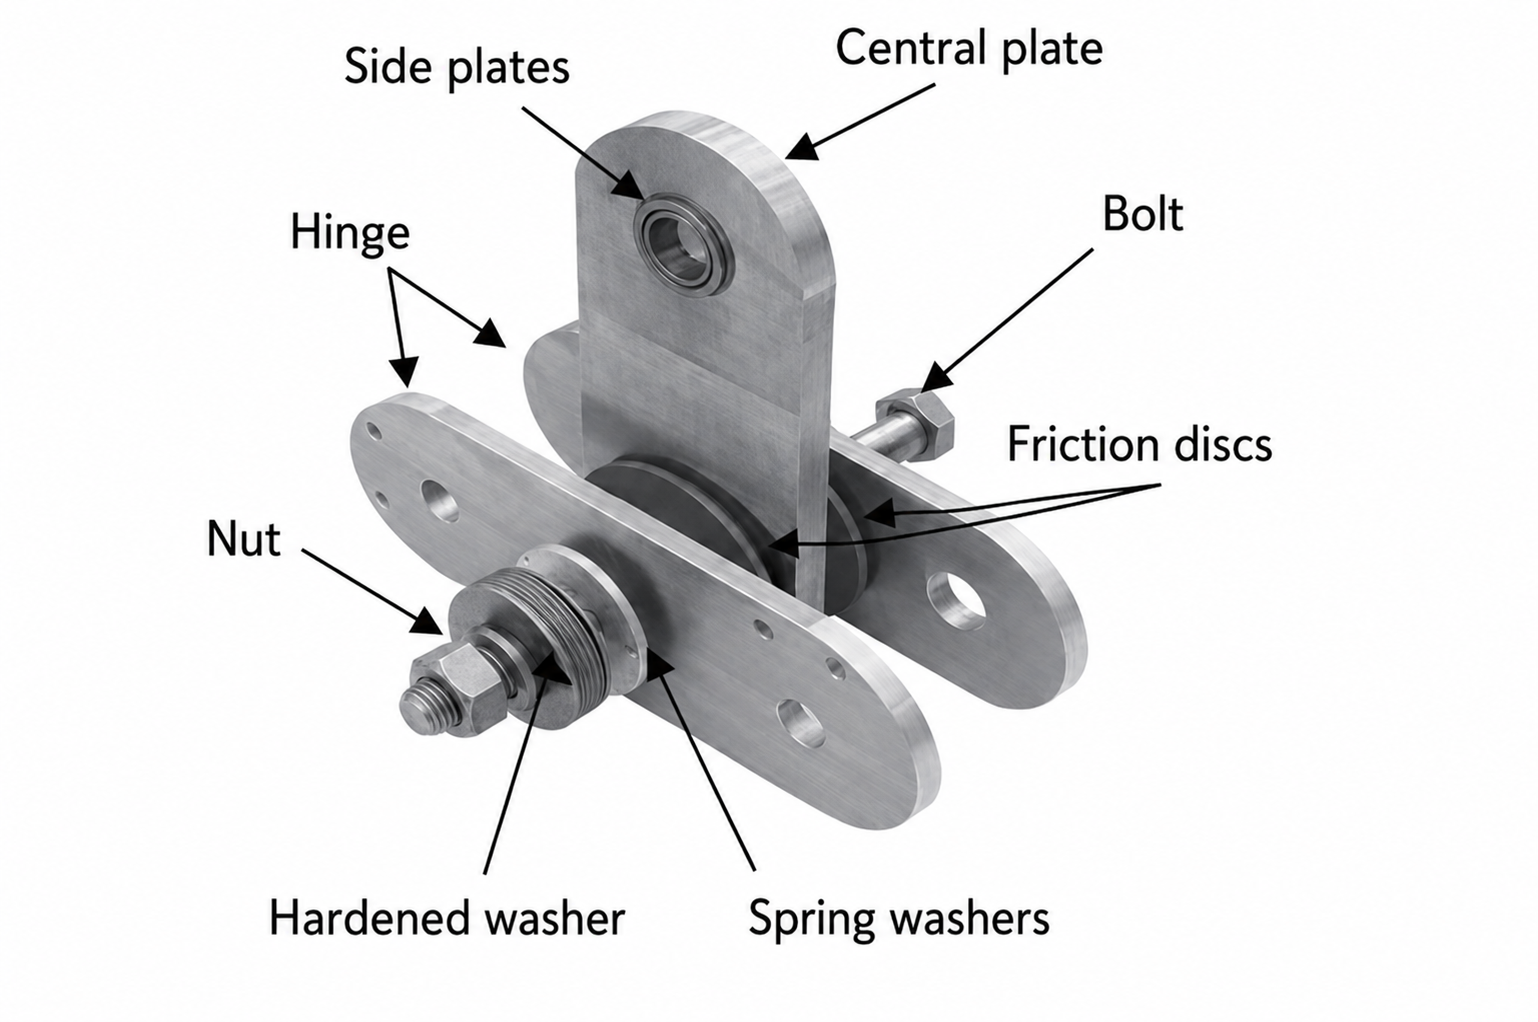
\includegraphics[width=\textwidth]{rfd_componentes.png}
        \caption{RFD components: central plate, lateral plates,
                 friction disks, prestressed bolt, and washers.}
        \label{fig:rfd_componentes}
    \end{subfigure}
    \hfill
    \begin{subfigure}[b]{0.48\textwidth}
        \centering
        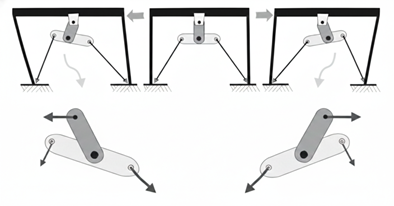
\includegraphics[width=\textwidth]{rfd_mecanismo.png}
        \caption{Actuation mechanism: lateral frame displacement induces
                 rotation in the device, dissipating energy through friction.}
        \label{fig:rfd_mecanismo}
    \end{subfigure}
    \caption{Rotational Friction Damper (RFD). Left: physical device configuration \citep{Mualla2002}.
             Right: activation sequence under lateral seismic excitation.}
    \label{fig:rfd}
\end{figure}

In a typical installation, the central plate of the RFD is connected to the midspan of the beam
through a pinned connection, while the lateral plates are linked to an inverted-V bracing system.
When the frame experiences lateral displacement due to seismic excitation, relative motion between
stories induces rotation in the device, as illustrated in Figure~\ref{fig:rfd_mecanismo}. This rotation
produces sliding between steel plates and friction disks, generating a resisting moment that opposes
motion. In this manner, part of the energy that would otherwise be dissipated through damage in the
primary frame members is transferred to the frictional device \citep{kim_use_2011}.

The friction capacity of the RFD is represented by the maximum frictional moment $\Mf$, which depends
on the applied normal force, coefficient of friction, and device geometry. The equivalent lateral
force transferred to the frame is:
\begin{equation}
    F_{\mathrm{afr}} = \frac{\Mf}{\ha},
    \label{eq:Fafr}
\end{equation}
where $\ha$ is the lever arm associated with the geometry of the bracing system. Experimentally,
\citet{Mualla2002} observed that the moment-rotation behavior of the device is virtually independent
of frequency in the 2--7\,Hz range, supporting the use of Coulomb friction law.

\subsection{Nonlinear Dynamic Analysis via Nonsmooth Dynamics}
\label{sec:theory:dns}

Coulomb friction presents a particularity that complicates its numerical integration: device behavior
changes abruptly between two states, slip ($|\dot{\varphi}|>0$) and stick ($\dot{\varphi}=0$), without
continuous transition between them. Conventional step-by-step integrators assume that forces vary
smoothly between instants, an assumption not satisfied for dry friction \citep{chopra_dynamics_2015}.
To handle this behavior without resorting to equivalent linearization, this work adopts the Nonsmooth
Dynamics (NSD) method proposed by \citet{Namorado2024}, which formulates the problem in terms of
velocities and impulses rather than instantaneous accelerations and forces.

\subsubsection*{Friction law}

For an RFD installed between stories $i$ and $i+1$, the relation between the resisting moment of the
device and the relative angular velocity $\dot{\varphi}_i$ follows Coulomb's law:
\begin{equation}
    M_{\mathrm{afr},i} \in -\Mf \cdot \operatorname{Sign}\!\left(\dot{\varphi}_i\right),
    \label{eq:coulomb}
\end{equation}
where $\operatorname{Sign}(\cdot)$ is the extended sign operator for the case of zero velocity:
\begin{equation}
    \operatorname{Sign}(v) =
    \begin{cases}
        \{+1\}    & \text{if } v > 0, \\
        [-1,\,+1] & \text{if } v = 0, \\
        \{-1\}    & \text{if } v < 0.
    \end{cases}
    \label{eq:sign}
\end{equation}
When the device slips ($|\dot{\varphi}_i|>0$) the moment equals exactly $\pm\Mf$; when at rest
($\dot{\varphi}_i=0$) the moment can take any value between $-\Mf$ and $+\Mf$ as required by static
equilibrium at that instant.

\subsubsection*{Equation of motion}

The system of $\np$ stories with $n_a$ installed dampers is governed, in continuous form, by the
differential inclusion \citep{Namorado2024}:
\begin{equation}
    \bm{M}\,\ddot{\bm{u}} + \bm{C}\,\dot{\bm{u}} + \bm{K}\,\bm{u}
    \in -\bm{M}\,\bm{r}\,\ddot{x}_g(t) + \bm{H}\,\bm{Q}_f(t),
    \label{eq:eom}
\end{equation}
where $\bm{M}$, $\bm{C}$, and $\bm{K}$ are the mass, damping, and stiffness matrices; $\bm{u}$ is
the vector of ground-relative displacements; $\bm{r}$ is the seismic influence vector; $\ddot{x}_g$
is ground acceleration; and $\bm{H}$ is a localization matrix indicating which stories have each
device installed ($+1$ on the upper story, $-1$ on the lower). The symbol $\in$ reflects that the
friction force $\bm{Q}_f(t)$ is \textit{multivalued}: during slip it takes the value $\pm\Mf/\ha$,
but during stick can take any value in the interval $[-\Mf/\ha,\,+\Mf/\ha]$ as required by equilibrium,
corresponding to Coulomb's law (Eq.~\ref{eq:coulomb}).

In the discrete implementation, the multivalued force $\bm{Q}_f$ is replaced by frictional impulses
$\bm{\lambda}_{k+1}$ computed at each step via solving a Linear Complementarity Problem (LCP, Eq.~\ref{eq:lcp}).
Once $\bm{\lambda}_{k+1}$ is determined, the force value is uniquely fixed for that step and the
inclusion becomes an equality:
\begin{equation}
    \bm{M}\,\ddot{\bm{u}} + \bm{C}\,\dot{\bm{u}} + \bm{K}\,\bm{u}
    = -\bm{M}\,\bm{r}\,\ddot{x}_g(t) + \bm{H}\,\bm{\lambda}_{k+1}/\Delta t.
    \label{eq:eom_disc}
\end{equation}
The equivalent frictional force recovered for story $i$ is
$f_{\mathrm{afr},i} = \lambda_i / (\ha\,\Delta t)$.

\subsubsection*{NSD-LCP-PSOR Integration Procedure}

Starting from the known state at instant $k$, the algorithm computes the state at $k+1$ in three
steps summarized in Algorithm~\ref{alg:nsd-lcp-psor}.

\textbf{Predictor.}
First, the velocity the system would have if dampers exerted no force in this step is calculated.
For this, a modified mass matrix is defined:
\begin{equation}
    \hat{\bm{M}} = \bm{M}
                  + \theta\Delta t\,\bm{C}
                  + (\theta\Delta t)^{2}\bm{K},
    \label{eq:Mhat}
\end{equation}
which groups inertias, damping, and stiffness into a single discrete-level operator. The friction-free
velocity is:
\begin{equation}
    \dot{\bm{u}}^{\mathrm{libre}} = \hat{\bm{M}}^{-1}
    \!\left[
        \bm{A}\,\dot{\bm{u}}_k
        - \Delta t\,\bm{K}\bm{u}_k
        - \theta\Delta t\,\bm{M}\!\left(\ddot{x}_{g,k+1}+\ddot{x}_{g,k}\right)\bm{r}
    \right],
    \label{eq:vfree}
\end{equation}
where $\bm{A} = \bm{M} - \theta\Delta t\,\bm{C} - (\theta\Delta t)^{2}\bm{K}$.
This result is equivalent to standard Newmark integration without considering friction forces.

\textbf{Corrector.}
In general, the free velocity does not satisfy Coulomb's condition: some dampers appear with nonzero
relative velocity when they should be at rest. The corrector determines the frictional impulses
$\bm{\lambda}_{k+1}$ necessary to simultaneously satisfy system dynamics and Coulomb's law limits.
For this, the free relative velocity at each damper is computed,
$q_r = \dot{u}^{\mathrm{libre}}_{f_r} - \dot{u}^{\mathrm{libre}}_{f_r-1}$,
and the coupling matrix between devices is constructed:
\begin{equation}
    W_{rs} = \left[\bm{H}^{\top}\hat{\bm{M}}^{-1}\bm{H}\right]_{rs}\Delta t,
    \label{eq:W}
\end{equation}
whose coefficients reflect how the impulse of one damper affects the relative velocity of others
through the structure. The impulses are obtained by solving the system:
\begin{equation}
    \bm{W}\bm{\lambda} + \bm{q} = \bm{0},
    \quad |\lambda_r| \leq \frac{\Mf\,\Delta t}{\ha},
    \quad r = 1,\ldots,n_a,
    \label{eq:lcp}
\end{equation}
which is a Linear Complementarity Problem (LCP) with box constraints. When a damper's impulse reaches
the limit $\Mf\Delta t/\ha$, the device is slipping; when below, it is stuck. The system is solved
iteratively via PSOR (\textit{Projected Successive Over-Relaxation}), updating each impulse in
sequence and projecting it onto the admissible interval until convergence.

\textbf{State update.}
With the computed impulses, velocity is corrected and displacement is advanced:
\begin{align}
    \dot{\bm{u}}_{k+1} &= \dot{\bm{u}}^{\mathrm{libre}}
        + \Delta t\,\hat{\bm{M}}^{-1}\bm{H}\bm{\lambda}_{k+1}, \label{eq:vupdate}\\
    \bm{u}_{k+1} &= \bm{u}_k
        + \Delta t\!\left[(1-\theta)\,\dot{\bm{u}}_k
                         + \theta\,\dot{\bm{u}}_{k+1}\right]. \label{eq:uupdate}
\end{align}
The impulse $\bm{\lambda}_{k+1}$ is reused as the starting point for PSOR in the next step, taking
advantage of the fact that friction response changes little between consecutive instants.

\begin{algorithm}[t]
\caption{NSD-LCP-PSOR applied to MDOF frames with RFD}
\label{alg:nsd-lcp-psor}
\begin{algorithmic}[1]
\Require $\bm{M},\bm{C},\bm{K}$; $\bm{H}$, $\bm{F}^{\lim}$;
         $\{\ddot{x}_{g,k}\}_{k=0}^{n}$; $\Delta t$, $\theta$
\Ensure  $\{\bm{u}_k,\dot{\bm{u}}_k\}_{k=0}^{n}$

\vspace{2pt}
\State \textit{// Pre-computation (once only)}
\State $\hat{\bm{M}} \leftarrow \bm{M} + \theta\Delta t\,\bm{C} + (\theta\Delta t)^{2}\bm{K}$
\State $\bm{A} \leftarrow \bm{M} - \theta\Delta t\,\bm{C} - (\theta\Delta t)^{2}\bm{K}$
\State $\bm{W} \leftarrow \left(\bm{H}^{\top}\hat{\bm{M}}^{-1}\bm{H}\right)\Delta t$
\State $\bm{u}_0 \leftarrow \bm{0}$;\quad $\dot{\bm{u}}_0 \leftarrow \bm{0}$;\quad
       $\bm{\lambda}_0 \leftarrow \bm{0}$

\vspace{2pt}
\For{$k = 0, 1, \ldots, n-1$}
    \vspace{2pt}
    \State \textit{// Step 1 — free velocity (friction-free predictor)}
    \State $\bm{b}_k \leftarrow \bm{A}\,\dot{\bm{u}}_k
            - \Delta t\,\bm{K}\bm{u}_k
            - \theta\Delta t\,\bm{M}
              \!\left(\ddot{x}_{g,k+1}+\ddot{x}_{g,k}\right)\bm{r}$
    \State $\dot{\bm{u}}^{\mathrm{lib}} \leftarrow \hat{\bm{M}}^{-1}\bm{b}_k$

    \vspace{2pt}
    \State \textit{// Step 2 — free relative velocities at each damper}
    \State $q_r \leftarrow \dot{u}^{\mathrm{lib}}_{f_r} - \dot{u}^{\mathrm{lib}}_{f_r-1}$
           \quad for $r = 1,\ldots,n_a$

    \vspace{2pt}
    \State \textit{// Step 3 — LCP resolution via PSOR (corrector)}
    \State $\bm{\lambda}^{(0)} \leftarrow \bm{\lambda}_k$
           \quad\textit{(starting point from previous step)}
    \While{$\|\bm{\lambda}^{(i+1)} - \bm{\lambda}^{(i)}\|_\infty > \varepsilon$}
        \For{$r = 1,\ldots,n_a$}
            \State $\tilde{\lambda}_r \leftarrow
                   -\!\left(q_r + \sum_{s \neq r} W_{rs}\lambda_s^{(i)}\right)\!\big/W_{rr}$
            \State $\lambda_r^{(i+1)} \leftarrow
                   \max\!\left(-F^{\lim}_r,\;\min\!\left(F^{\lim}_r,\;\tilde{\lambda}_r\right)\right)$
        \EndFor
    \EndWhile
    \State $\bm{\lambda}_{k+1} \leftarrow \bm{\lambda}^{(*)}$
           \quad\textit{($F^{\lim}_r = \Mf\Delta t/\ha$)}

    \vspace{2pt}
    \State \textit{// Step 4 — state update}
    \State $\dot{\bm{u}}_{k+1} \leftarrow
           \dot{\bm{u}}^{\mathrm{lib}} +
           \Delta t\,\hat{\bm{M}}^{-1}\bm{H}\bm{\lambda}_{k+1}$
    \State $\bm{u}_{k+1} \leftarrow \bm{u}_k +
           \Delta t\!\left[(1-\theta)\,\dot{\bm{u}}_k +
                           \theta\,\dot{\bm{u}}_{k+1}\right]$
\EndFor
\end{algorithmic}
\end{algorithm}

The time step used, $\Delta t = 0.01$\,s, corresponds to the native sampling interval of the seismic
records, avoiding input signal interpolation. For the stiffest structures in the experiment
($T_1 = 0.3$\,s) this represents approximately 30 integration points per period, satisfying the standard
criterion $\Delta t / T_1 \leq 0.10$ recommended for Newmark methods \citep{chopra_dynamics_2015}.
The equivalent frictional force at story $i$ is recovered as:
\begin{equation}
    f_{\mathrm{afr},i} = \frac{\lambda_i}{\ha\,\Delta t},
    \label{eq:ffrict}
\end{equation}
so that the slip or stick state of each device is determined automatically by LCP solution, without
explicit detection.

\subsubsection*{Adaptation of NSD Method for Massive MDOF Simulation}
\label{sec:theory:nsd:adaptacion}

The NSD method of \citet{Namorado2024} was developed and validated for frames of one to five stories
with one damper per story. This work applies it to frames of up to twenty stories with variable damper
configurations, requiring three adjustments to the original algorithm.

\textbf{LCP formulation of the corrector.}
Rather than updating impulses of each damper separately in sequence, all are solved jointly via the
matrix $\bm{W}$ (Eq.~\ref{eq:W}), capturing how different devices interact through the structure.
This is more direct when several dampers are active simultaneously on different stories, though it
requires computing $\hat{\bm{M}}^{-1}$ once before starting integration.

\textbf{No tuning parameter.}
The original algorithm includes a parameter $\alpha$ controlling convergence speed of the corrector
and which must be chosen for each case. By formulating the problem as LCP, this parameter disappears:
the iterative procedure converges without manual adjustment, facilitating application to the thousands
of distinct configurations in the experiment.

\textbf{Impulse reuse between steps.}
The impulse computed at step $k$ is used as the starting point at step $k+1$. Since system response
changes gradually, this initial value is usually near the solution, requiring fewer iterations to
converge.

In physical terms, the two formulations are equivalent: both solve the same discrete Coulomb friction
law. The difference lies in how the computation is organized to efficiently handle the larger number
of stories and dampers in this study.

\subsection{Seismic Performance Metric}
\label{sec:theory:metrica}

The seismic performance of each RFD configuration is quantified via normalized response ratios relative
to the reference bare frame, an approach consistent with prior RFD work \citep{Namorado2024, Jarrahi2020jbe, Mualla2002}.
For each configuration--record pair, three ratios are computed:
\begin{equation}
    R_1 = \frac{u_{\max}^{(c)}}{u_{\max}^{(0)}}, \quad
    R_2 = \frac{\ddot{u}_{\max}^{(c)}}{\ddot{u}_{\max}^{(0)}}, \quad
    R_3 = \frac{V_{\max}^{(c)}}{V_{\max}^{(0)}},
    \label{eq:R_individual}
\end{equation}
where superscripts (c) and (0) denote controlled and uncontrolled structure, respectively; $u_{\max}$
is maximum roof displacement, $\ddot{u}_{\max}$ is maximum absolute acceleration, and $V_{\max}$ is
maximum base shear. From $R_1$, $R_2$, and $R_3$, two composite indices are constructed using
Euclidean norm. The first combines displacement and acceleration:
\begin{equation}
    CR_1 = \sqrt{R_1^2 + R_2^2},
    \label{eq:CR1}
\end{equation}
and the second adds base shear, integrating all three response aspects simultaneously:
\begin{equation}
    CR_2 = \sqrt{R_1^2 + R_2^2 + R_3^2}.
    \label{eq:CR2}
\end{equation}
When dampers have no effect, $R_1 = R_2 = R_3 = 1$ and thus $CR_2 = \sqrt{3}$; smaller values indicate
that the configuration reduces seismic response in some combination of the three measures.

Since seismic response depends on the record considered, $CR_2$ is computed for each configuration--record
pair. Following standard practice in performance-based seismic evaluation \citep{Kazemi2022}, the value
of $CR_2$ is summarized across $N_r = 8$ records using three percentile statistics:
\begin{align}
    \CR{P10} &= Q_{0.10}\!\left(\{CR_2^{(k)}\}_{k=1}^{N_r}\right), \quad
    \CR{med}  = Q_{0.50}\!\left(\{CR_2^{(k)}\}_{k=1}^{N_r}\right), \notag\\
    \CR{P90} &= Q_{0.90}\!\left(\{CR_2^{(k)}\}_{k=1}^{N_r}\right),
    \label{eq:CR2stats}
\end{align}
where $Q_p$ denotes the $p$-th quantile. These three statistics serve as target variables for the ML
models. The interpretation is: $\CR{P10}$ represents a favorable response condition, $\CR{med}$ describes
typical behavior, and $\CR{P90}$ approximates a severe condition within the record set, enabling distinction
between configurations that only perform adequately under one particular record from those with stable
performance across seismic variability.

\subsection{Machine Learning for Structural Optimization}
\label{sec:theory:ml}

Optimization of passive dissipation systems involves seeking the optimal combination of location, number,
and capacity of devices to minimize some indicator of seismic response. Prior approaches have addressed
this problem using energy methods and metaheuristic algorithms applied to conventional and rotational
friction dampers \citep{moreschi_design_2003, moghaddam_optimal_2022, ontiveros-perez_reliability-based_2019}.
Machine learning enables construction of surrogate models approximating the input--output relation of
nonlinear analysis at significantly lower computational cost, enabling efficient exploration of high-dimensional
design spaces.

In the surrogate model paradigm, a regression function $\hat{y} = f(\bm{x};\,\bm{\theta})$ is trained on data
$\{(\bm{x}_i,\,y_i)\}_{i=1}^{N}$ to approximate the mapping between design variables $\bm{x}$ (structural
and RFD parameters) and target variable $y$ (one of the three $CR_2$ statistics). Training minimizes mean
squared error:
\begin{equation}
    \mathcal{L}(\bm{\theta}) = \frac{1}{N}\sum_{i=1}^{N}
    \bigl(y_i - f(\bm{x}_i;\,\bm{\theta})\bigr)^2.
    \label{eq:mse}
\end{equation}

Four algorithms are compared: (i)~Linear Regression and (ii)~Ridge Regression ($\ell_2$ penalization)
as linear baselines; (iii)~Random Forest \citep{Breiman2001}, averaging predictions from multiple
independently-trained trees; and (iv)~XGBoost \citep{Chen2016}, a gradient boosting algorithm that
sequentially corrects residuals of a growing ensemble. Generalization is estimated via five-fold
GroupKFold cross-validation \citep{Kazemi2022}, where groups correspond to unique structure identifiers.
This strategy prevents different configurations of the same building ---sharing dynamic properties and
thus correlated responses--- from appearing simultaneously in training and validation, avoiding performance
overestimation via information leakage between folds. Evaluation metrics are:
\begin{equation}
    \RMSE = \sqrt{\frac{1}{|V|}\sum_{i \in V}\bigl(y_i - \hat{y}_i\bigr)^2},
    \qquad
    \Rsq  = 1 - \frac{\sum_{i \in V}(y_i - \hat{y}_i)^2}
                      {\sum_{i \in V}(y_i - \bar{y})^2},
    \label{eq:metrics}
\end{equation}
where $V$ is the validation set, $\hat{y}_i$ are out-of-fold predictions, and $\bar{y}$ is the mean of
observed values.

%%═══════════════════════════════════════════════════════════════════════════
\section{Methodology}
\label{sec:method}
%%═══════════════════════════════════════════════════════════════════════════

\subsection{Design of Experiments}
\label{sec:method:doe}

Latin Hypercube Sampling (LHS) \citep{McKay1979} was used to generate 1,000 structurally diverse
shear-type frames. Each configuration is defined by five structural variables: number of stories
$\np \in \{3, 5, 7, 10, 12, 15, 18, 20\}$; target fundamental period $T_1 \in [0.3,\,3.0]$\,s;
average mass per level $\bar{m} \in [150,\,350]$\,t/story; mass distribution profile (uniform, linear
ascending, linear descending, or concentrated at top); and lateral stiffness profile (uniform, linear
ascending, linear descending, or soft story at base). Lateral stiffness was analytically calibrated to
satisfy the target $T_1$ via the generalized eigenvalue problem $(\bm{K} - \omega_1^2\,\bm{M})\,\bm{\phi}_1 = \bm{0}$,
with $\omega_1 = 2\pi/T_1$.

For each structure, approximately 50 RFD configurations were generated: 40 via LHS over binary location space
and frictional moment range $\Mf \in [25,\,500]$\KM, and 10 structured configurations targeting specific
coverage fractions. Configuration is encoded via binary vector $\bm{b} \in \{0,1\}^{\np}$, where $b_i = 1$
indicates RFD presence at story $i$, yielding damper count $\nd = \|\bm{b}\|_0$ and coverage density
$\etad = \nd/\np \in (0,\,1]$. The full experimental plan comprises 433,984 simulations
($\approx 1,000 \times 54 \times 8$).

\subsection{Structural Models and Dynamic Analysis}
\label{sec:method:modelo}

Each structure is modeled as a linear shear frame with concentrated masses per story and lateral stiffness
between stories. The diagonal mass matrix is $\bm{M} = \mathrm{diag}(m_1,\ldots,m_{\np})$ and the tridiagonal
stiffness matrix $\bm{K}$ is assembled from the inter-story stiffness vector $k_i$. Rayleigh damping is adopted
with ratio $\zeta = 3\%$, calibrated to modes 1 and 3 \citep{chopra_dynamics_2015}. The eight real accelerograms
constituting seismic demand are: El~Centro~1940, Jamiltepec~2018, Kobe~1995, Loma Prieta~1989, Niltepec~2017,
Northridge~1994, Trinidad~1983, and Zacatula~1997. Time-history integration follows the NSD midpoint scheme
\citep{Namorado2024} with time step $\Delta t = 0.01$\,s, equal to the native sampling interval of records.
The lever arm is fixed at $\ha = 0.40$\,m, a value within the range reported in literature for steel frames
with RFD \citep{Mualla2002, Jarrahi2020jbe}.

\subsection{Feature Engineering}
\label{sec:method:features}

The four primary design variables do not capture the spatial information of the RFD configuration nor the
scaling relations between parameters; a tree-based model trained only on them would have to infer quotients
and positions from components, increasing required depth and potentially degrading generalization. Five
derived features are therefore computed that explicitly encode this information.

The complete feature vector contains 29 predictors distributed across three groups:

\begin{enumerate}[label=\textit{\roman*})]
    \item \textbf{Primary design variables} (4):
          number of stories $\np$, target fundamental period $T_1$,
          frictional moment $\Mf$, and damper count $\nd$.

    \item \textbf{Derived features} (5):
    \begin{itemize}
        \item $\etad = \nd/\np$: damper density, dominant design variable per importance
              analysis (Section~\ref{sec:results:importancia});
        \item $\bar{p} = \tfrac{1}{\nd}\sum_{i:\,b_i=1} i$: average device position in story number;
        \item $\tilde{p} = \bar{p}/\np \in (0,\,1]$: normalized average position, indicator
              of whether RFDs are concentrated in lower or upper stories;
        \item $\sigma_p = \mathrm{std}\!\left(\{i:b_i=1\}\right)/\np$:
              normalized vertical dispersion, distinguishing uniform from clustered configurations;
        \item $\tilde{E} = E_{\mathrm{total}}/(\np\times10^6)$: normalized total dissipated
              energy per story, proxy for integrated dynamic demand.
    \end{itemize}

    \item \textbf{Binary location indicators} (20):
          $b_1,\ldots,b_{20}$, where $b_i=1$ if story $i$ has an RFD and $b_i=0$ otherwise;
          frames with fewer than 20 stories are padded with zeros.
\end{enumerate}

\subsection{Training and Validation}
\label{sec:method:entrenamiento}

The objectives $\CR{med}$, $\CR{P10}$, and $\CR{P90}$ are predicted independently. For each objective,
the four algorithms are trained and evaluated via five-fold GroupKFold cross-validation. Hyperparameters
are fixed to standard values: Random Forest uses $n=100$ trees and maximum depth 15; XGBoost uses $n=100$
estimators, maximum depth 6, and learning rate $\eta=0.1$. Feature importance is derived from mean impurity
decrease across all trees in the trained XGBoost model. Out-of-fold (OOF) predictions are assembled across
folds to compute reported values of $\RMSE$ and $\Rsq$.

%%═══════════════════════════════════════════════════════════════════════════
\section{Results}
\label{sec:results}
%%═══════════════════════════════════════════════════════════════════════════

\subsection{Predictive Performance of ML Models}
\label{sec:results:desempenio}

\Cref{tab:desempenio} presents RMSE and $R^2$ with cross-validation for all models and objectives.
Ensemble models achieve a 49\% reduction in $\RMSE$ compared to linear baselines for $\CR{med}$, and 40\%
for $\CR{P10}$. XGBoost obtains the lowest error in $\CR{med}$ and $\CR{P10}$, while Random Forest shows
a slight advantage in $\CR{P90}$ (\cref{fig:comparacion_modelos}).

\begin{table}[h!]
\centering
\caption{RMSE and $R^2$ with cross-validation by model and target variable.
         Five-fold GroupKFold, grouped by structure identifier.}
\label{tab:desempenio}
\small
\setlength{\tabcolsep}{4pt}
\begin{tabular}{lcccccc}
\toprule
& \multicolumn{2}{c}{$\CR{med}$}
& \multicolumn{2}{c}{$\CR{P10}$}
& \multicolumn{2}{c}{$\CR{P90}$} \\
\cmidrule(lr){2-3}\cmidrule(lr){4-5}\cmidrule(lr){6-7}
Model & $\RMSE$ & $\Rsq$ & $\RMSE$ & $\Rsq$ & $\RMSE$ & $\Rsq$ \\
\midrule
Linear Regression & 0.1274 & 0.695 & 0.1267 & 0.812 & 0.1838 & 0.435 \\
Ridge            & 0.1274 & 0.695 & 0.1268 & 0.812 & 0.1838 & 0.435 \\
Random Forest    & 0.0681 & 0.913 & 0.0785 & 0.928 & 0.0981 & \textbf{0.839} \\
XGBoost          & \textbf{0.0652} & \textbf{0.920} & \textbf{0.0755} & \textbf{0.933} & 0.0984 & 0.838 \\
\bottomrule
\end{tabular}
\end{table}

\begin{figure}[htbp]
\centering
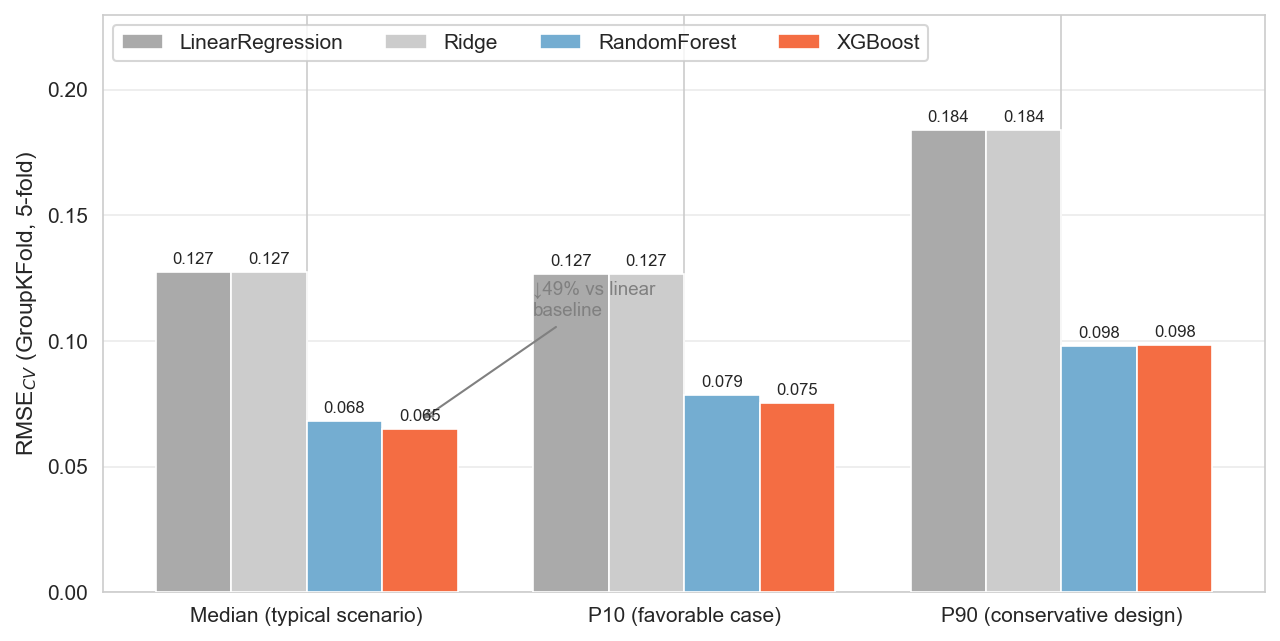
\includegraphics[width=0.85\linewidth]{figs/F1_model_comparison_rmse.png}
\caption{Comparison of cross-validation RMSE across models and target variables.
Ensemble models achieve approximately half the error of linear baselines.}
\label{fig:comparacion_modelos}
\end{figure}

For $\CR{P10}$ linear models achieve $\Rsq = 0.81$, indicating that in favorable scenarios, the
relationship between predictors and response is predominantly linear. The substantially lower $\Rsq = 0.44$
for $\CR{P90}$ under linear models confirms that the conservative scenario is governed by nonlinear
interactions that only ensemble models can capture.

\Cref{fig:pred_vs_actual} shows OOF scatter of XGBoost on $\CR{med}$, along with residual analysis.
Predictions distribute tightly around the identity line without systematic bias. A slight increase in
residual magnitude is observed for $CR_2 > 1.8$, a zone dominated by low-rise frames ($\np \leq 5$); in
these cases structural response is more sensitive to small parameter variations, increasing intrinsic target
variability and complicating prediction.

\begin{figure}[htbp]
\centering
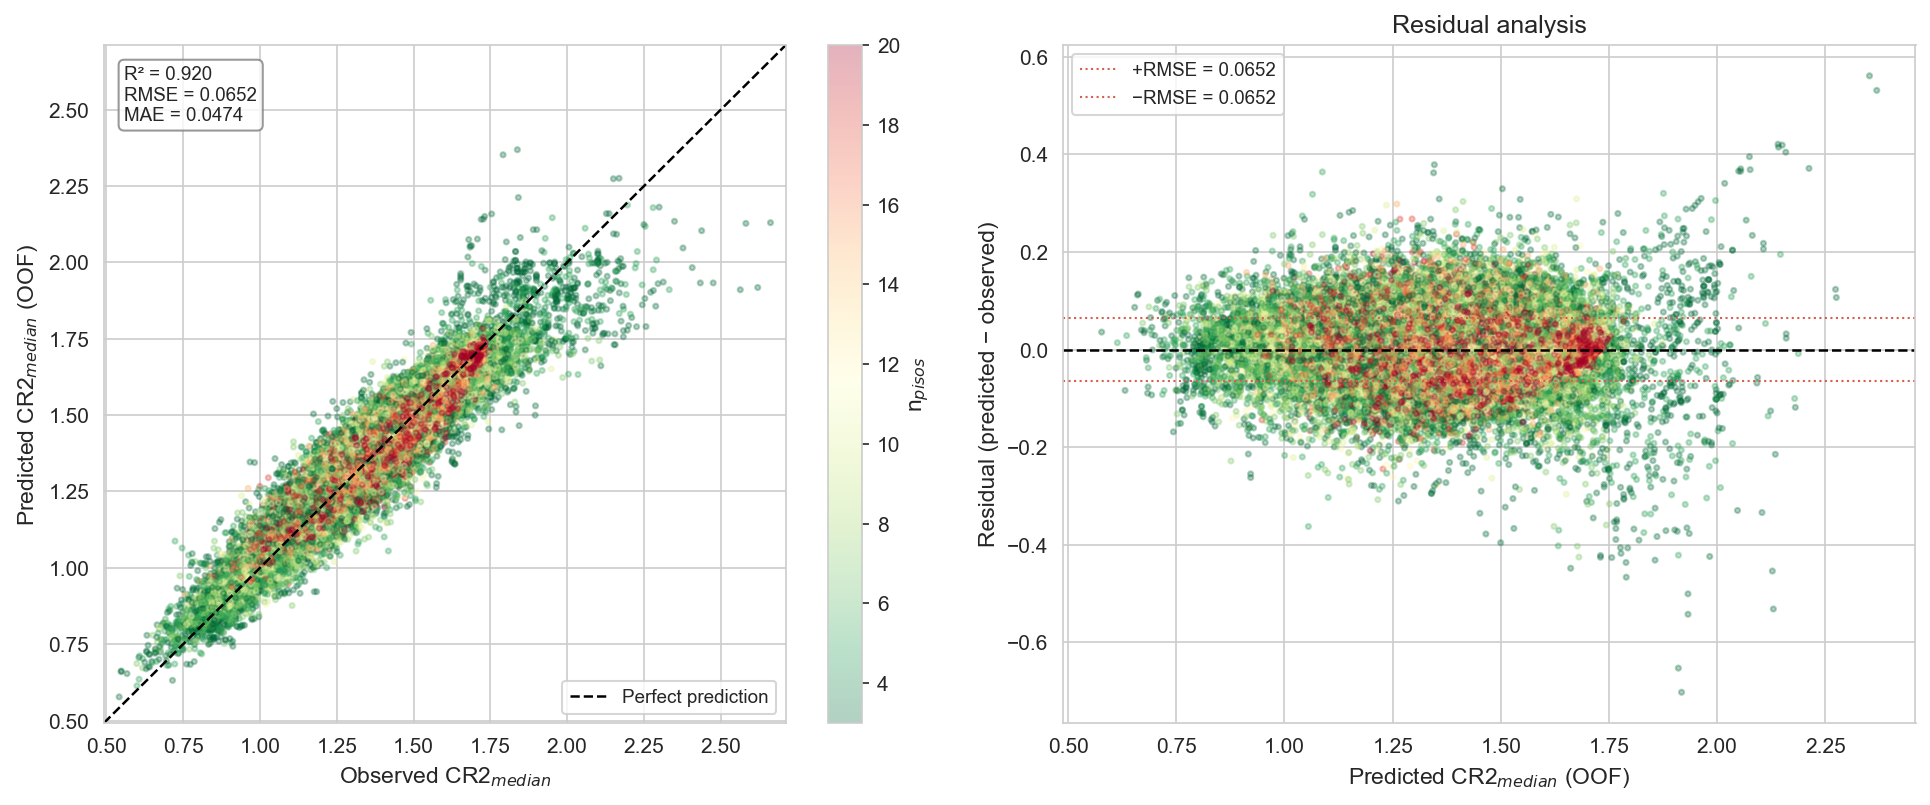
\includegraphics[width=\linewidth]{figs/F2_predicted_vs_actual_oof.png}
\caption{XGBoost OOF for $\CR{med}$. \textit{Left}: prediction vs.\ observed value;
dashed line: perfect prediction; color: $\np$. \textit{Right}: residuals (predicted $-$ observed)
vs.\ predicted; dashed bands: $\pm\RMSE$. $\Rsq = 0.92$, $\RMSE = 0.065$.}
\label{fig:pred_vs_actual}
\end{figure}

\begin{figure}[htbp]
\centering
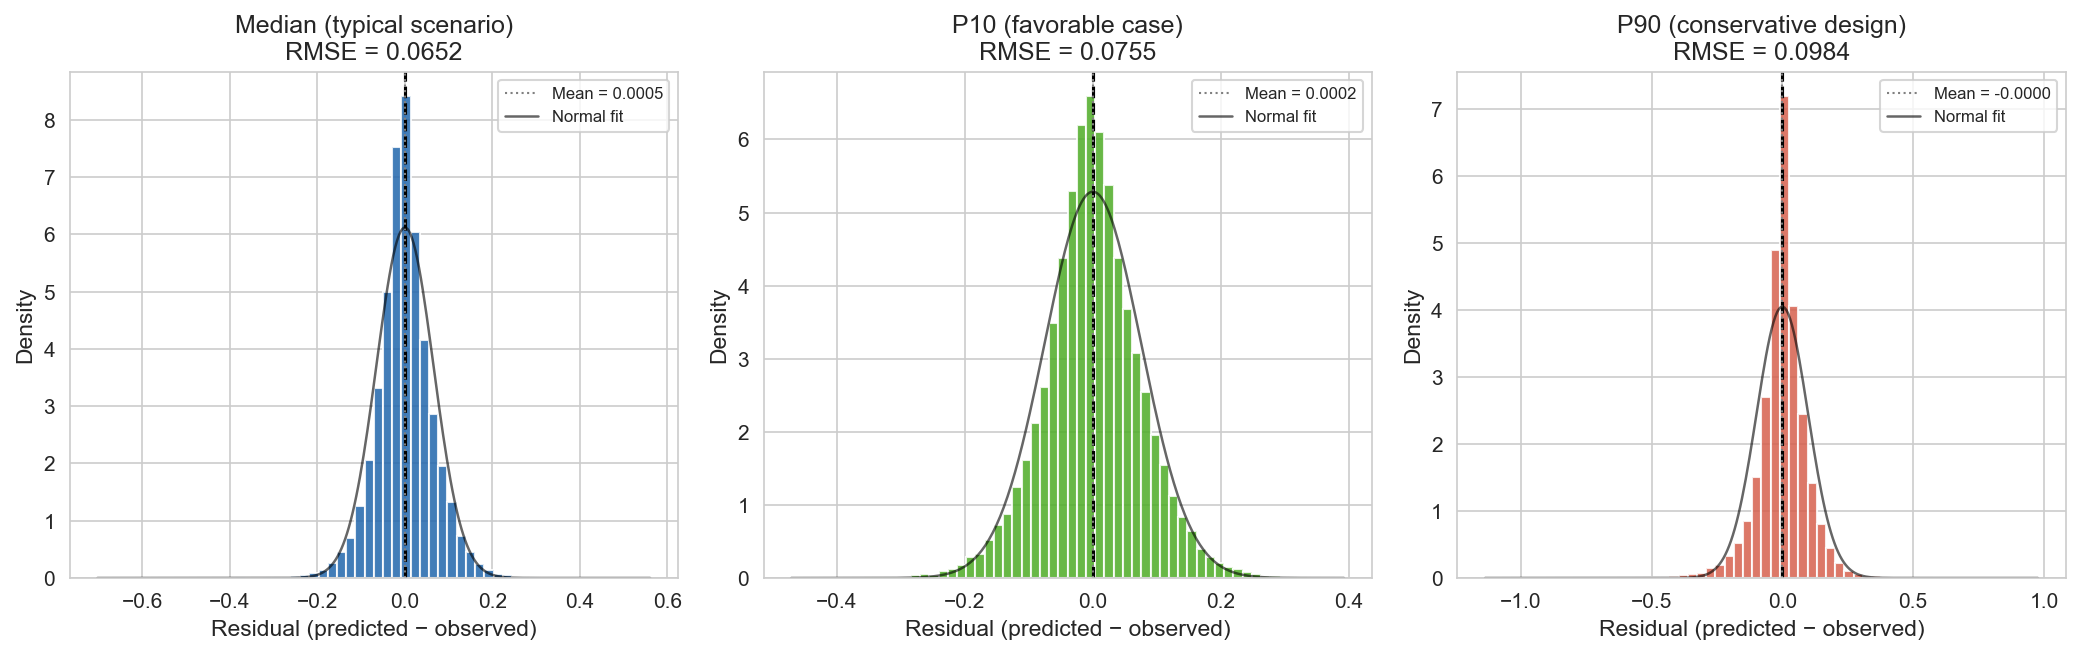
\includegraphics[width=\linewidth]{figs/F3_residual_distributions.png}
\caption{Residual distributions (OOF, XGBoost) for the three target variables of $CR_2$.
Dashed line: zero mean reference; solid curve: normal fit.}
\label{fig:residuales}
\end{figure}

\subsection{Design Variable Hierarchy and Feature Importance}
\label{sec:results:importancia}

\Cref{fig:importancia} presents the top 12 features for each target variable, derived from the
XGBoost model. Across all three scenarios, damper density $\etad$ consistently ranks first, with Pearson
correlation $r = -0.73$ with $\CR{med}$, versus $r = -0.45$ for absolute count $\nd$.

Normalized dissipated energy $\tilde{E}$ ($r = -0.70$) and vertical dispersion $\sigma_p$ ($r = -0.54$)
rank second and third, respectively, and are closely linked: homogeneous device distribution along height
favors more uniform energy dissipation across stories, reducing demand concentration at specific levels.
In particular, configurations including lower stories ---where inter-story drift is typically greatest---
prove more efficient, consistent with \citet{aydin_simple_2013} and optimization findings of
\citet{moghaddam_optimal_2022} and \citet{miguel_simultaneous_2016}. Frictional moment $\Mf$ shows
marginal weaker correlation ($r = -0.19$) in isolation, but interacts strongly with $\etad$, as shown
in \cref{sec:results:interaccion}.

A notable difference between scenarios is the behavior of $\CR{P90}$: global density $\etad$ loses its
dominant position (rank 1 in median and P10, rank 4 in P90) and is replaced by specific presence of
dampers in stories 1 and 2 along with building height $\np$, which occupy the top three ranks. This
indicates that under the most demanding records, precise location at lower levels and structural
characteristics gain greater relevance than global coverage.

\begin{figure}[htbp]
\centering
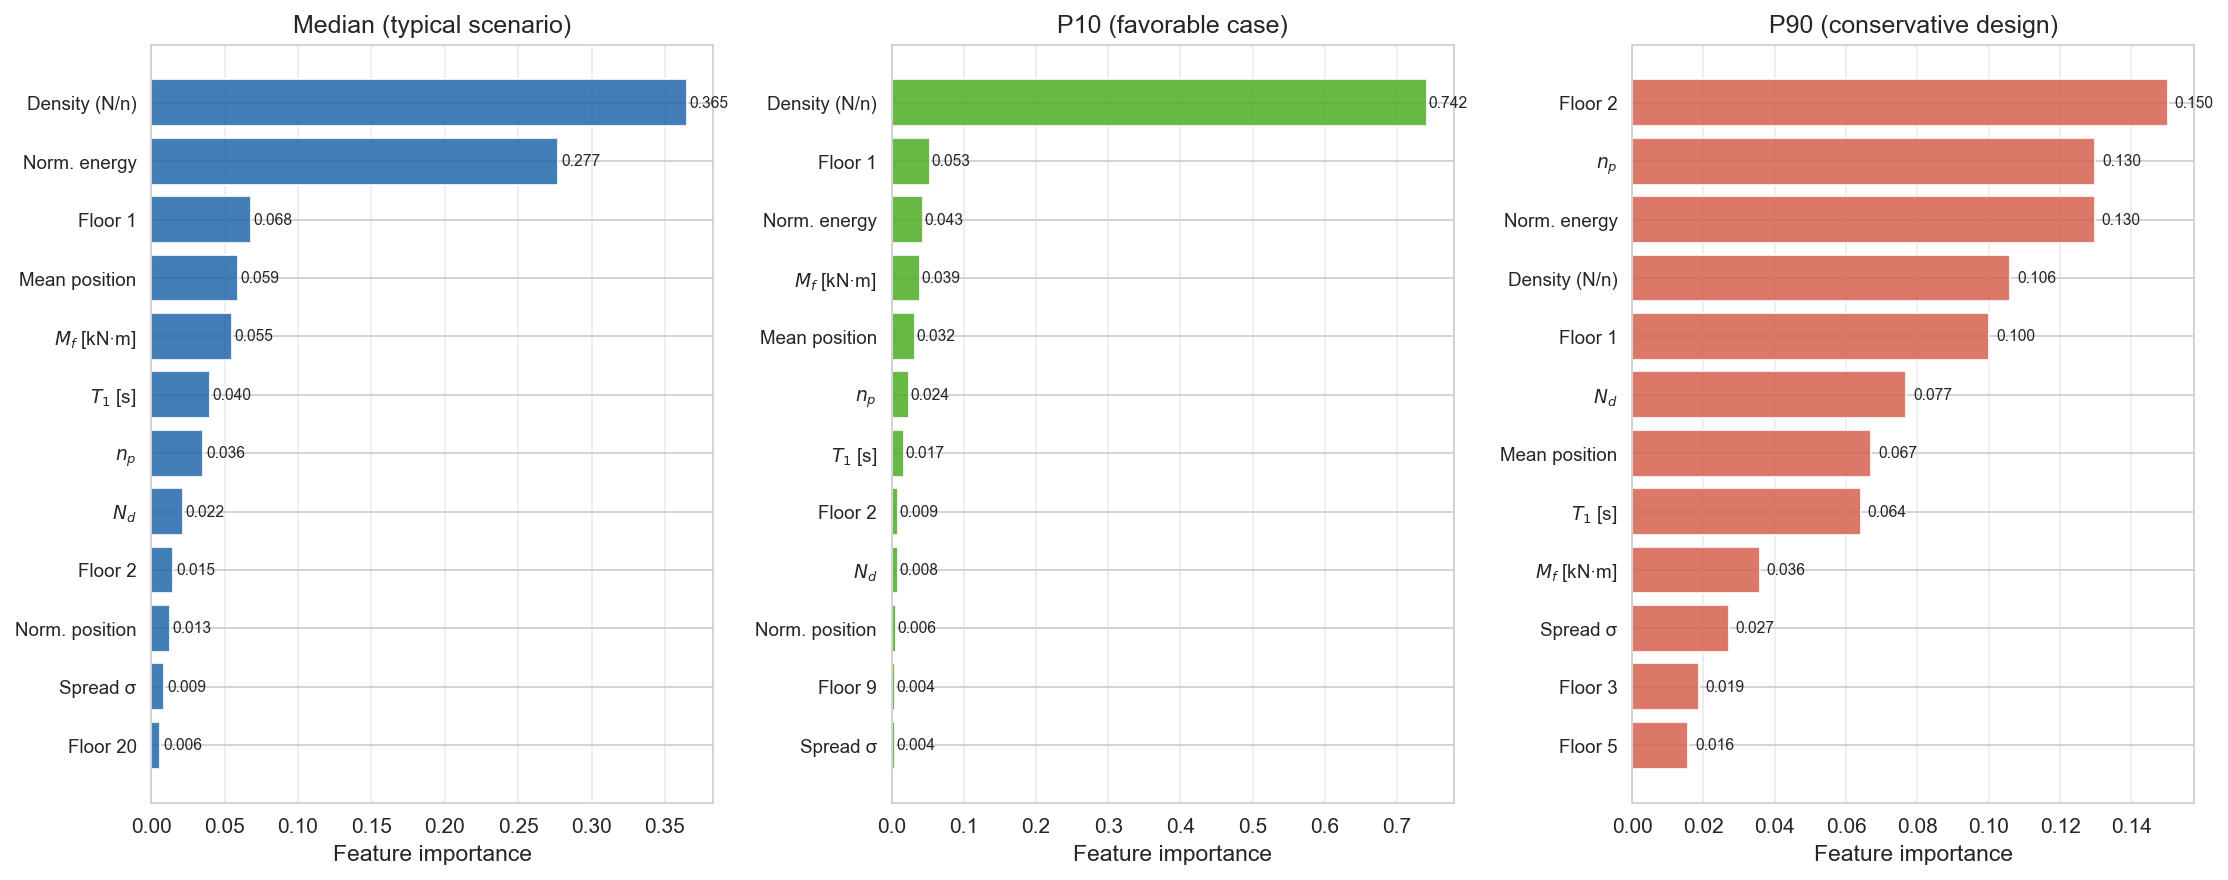
\includegraphics[width=\linewidth]{figs/F4_feature_importance_3targets.png}
\caption{Feature importance (XGBoost) for the top 12 predictors in the three $CR_2$ scenarios.
Horizontal bars indicate mean impurity decrease, normalized within each model. Note: horizontal axes
of each panel have independent scales; comparison between scenarios should be made by relative importance
rank, not absolute magnitude.}
\label{fig:importancia}
\end{figure}

\subsection{Diminishing Returns: Effect of Damper Density}
\label{sec:results:decreciente}

\Cref{fig:decreciente} investigates the diminishing returns relationship between $\etad$ and $CR_2$.
For each structure, the best $\CR{med}$ achievable was identified for each value of $\nd$, selecting the
minimum $CR_2$ among all configurations sharing that count. Performance curves are stratified by building
height to eliminate the confounding effect of $\np$ on the $\nd$ absolute axis.

The curves confirm a consistent diminishing returns pattern across all height categories, with steepest
improvement in the range $\etad \in [0.30,\,0.60]$. Beyond $\etad = 0.60$, marginal gain per additional
story covered decreases monotonically. A threshold analysis based on normalized intra-structure gain
(\cref{fig:curvas_internas}) indicates that 80\% of maximum performance improvement is achieved at
$\etad \approx 0.85$ for mid-rise (6--10 stories), high-rise (11--15 stories), and tall (16--20 stories)
frames. Low-rise frames (3--5 stories) require $\etad \approx 0.95$ to reach the same 80\% threshold,
attributed to the proportionally greater impact of each additional device in buildings with few stories.

To verify whether this dominance of $\etad$ holds independent of other design variables, stochastic
dominance analysis was performed on the eight seismic records separately. On each record, the 5th
percentile (best 5\%) of $CR_2$ in a higher density interval was compared against the 95th percentile
(worst 5\%) of the immediately lower interval. Dominance is confirmed across all eight records: even an
unfavorable configuration in $\Mf$, position, or $T_1$, but with greater coverage density, outperforms
95\% of configurations with lower density. Pearson correlation between $\etad$ and $CR_2$ ranges from
$r=-0.74$ (El~Centro~1940) to $r=-0.55$ (Kobe~1995) for most records. The exception is Trinidad~1983
($r=-0.18$), where correlation with density weakens notably and position and per-device capacity variables
recover relevance, suggesting that low-intensity or atypical frequency-content records can reduce
$\etad$ dominance.

\begin{figure}[htbp]
\centering
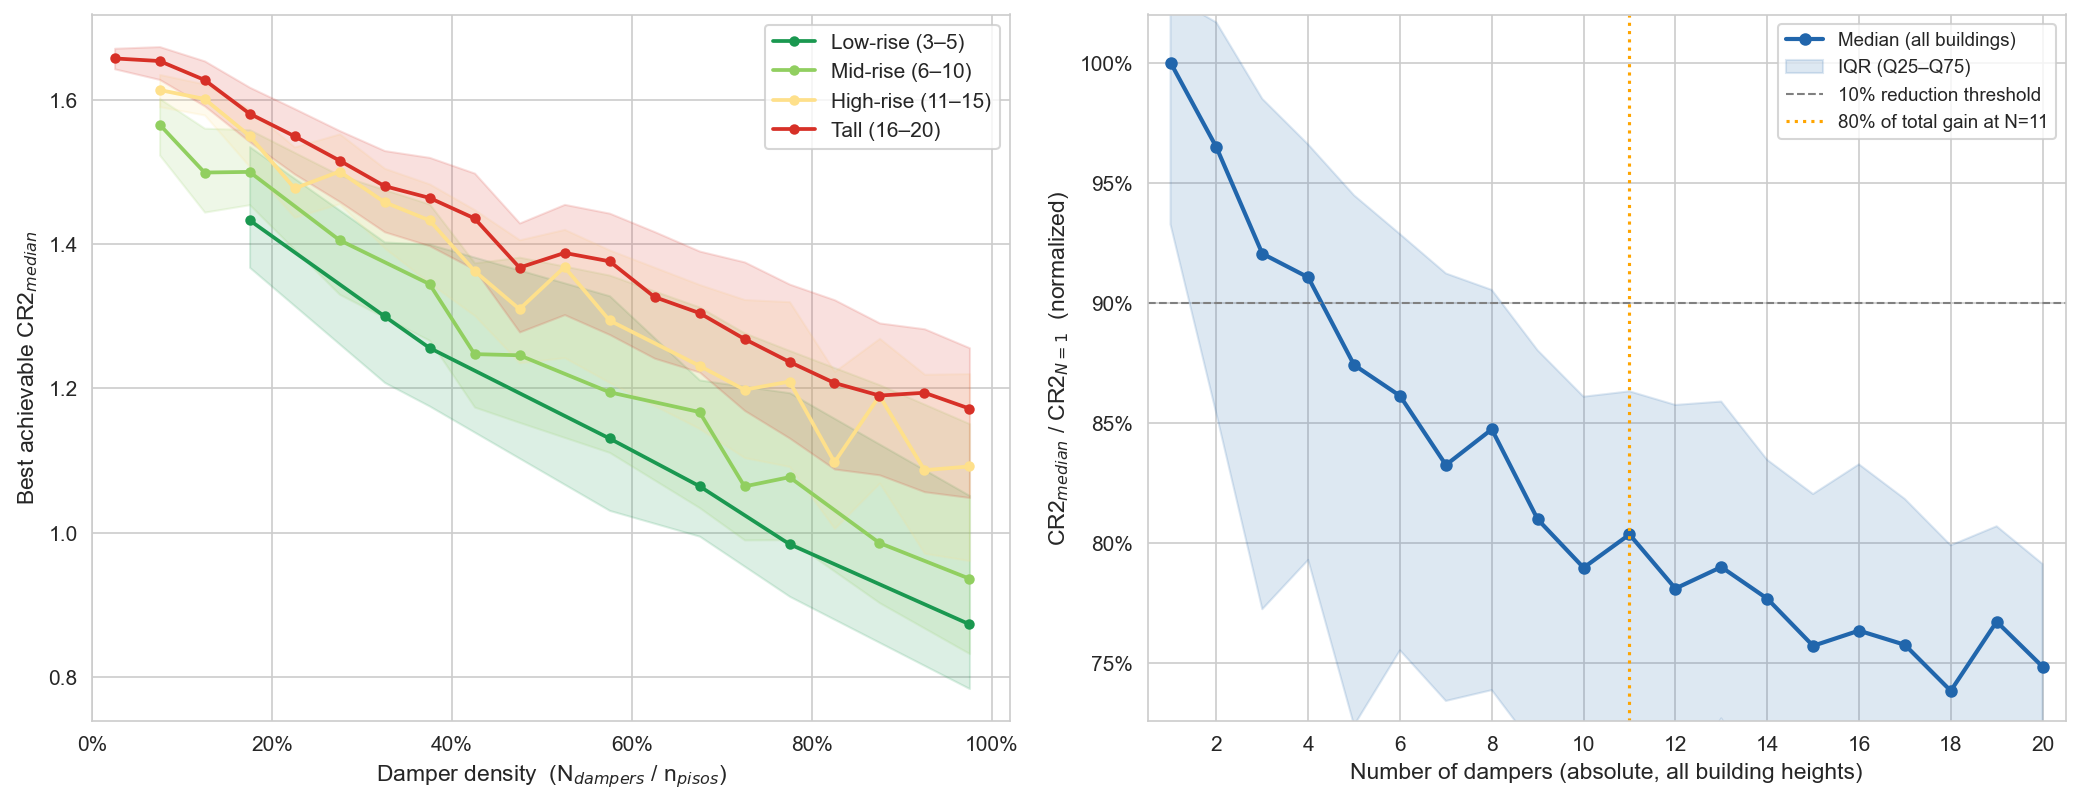
\includegraphics[width=\linewidth]{figs/F5_diminishing_returns.png}
\caption{Left: best achievable $\CR{med}$ vs.\ coverage density $\etad$, stratified by building height
(median $\pm$ IQR). Right: normalized $CR_2$ vs.\ absolute $\nd$ across all buildings (note: confounded
with height; left panel provides appropriate comparison).}
\label{fig:decreciente}
\end{figure}

\begin{figure}[htbp]
\centering
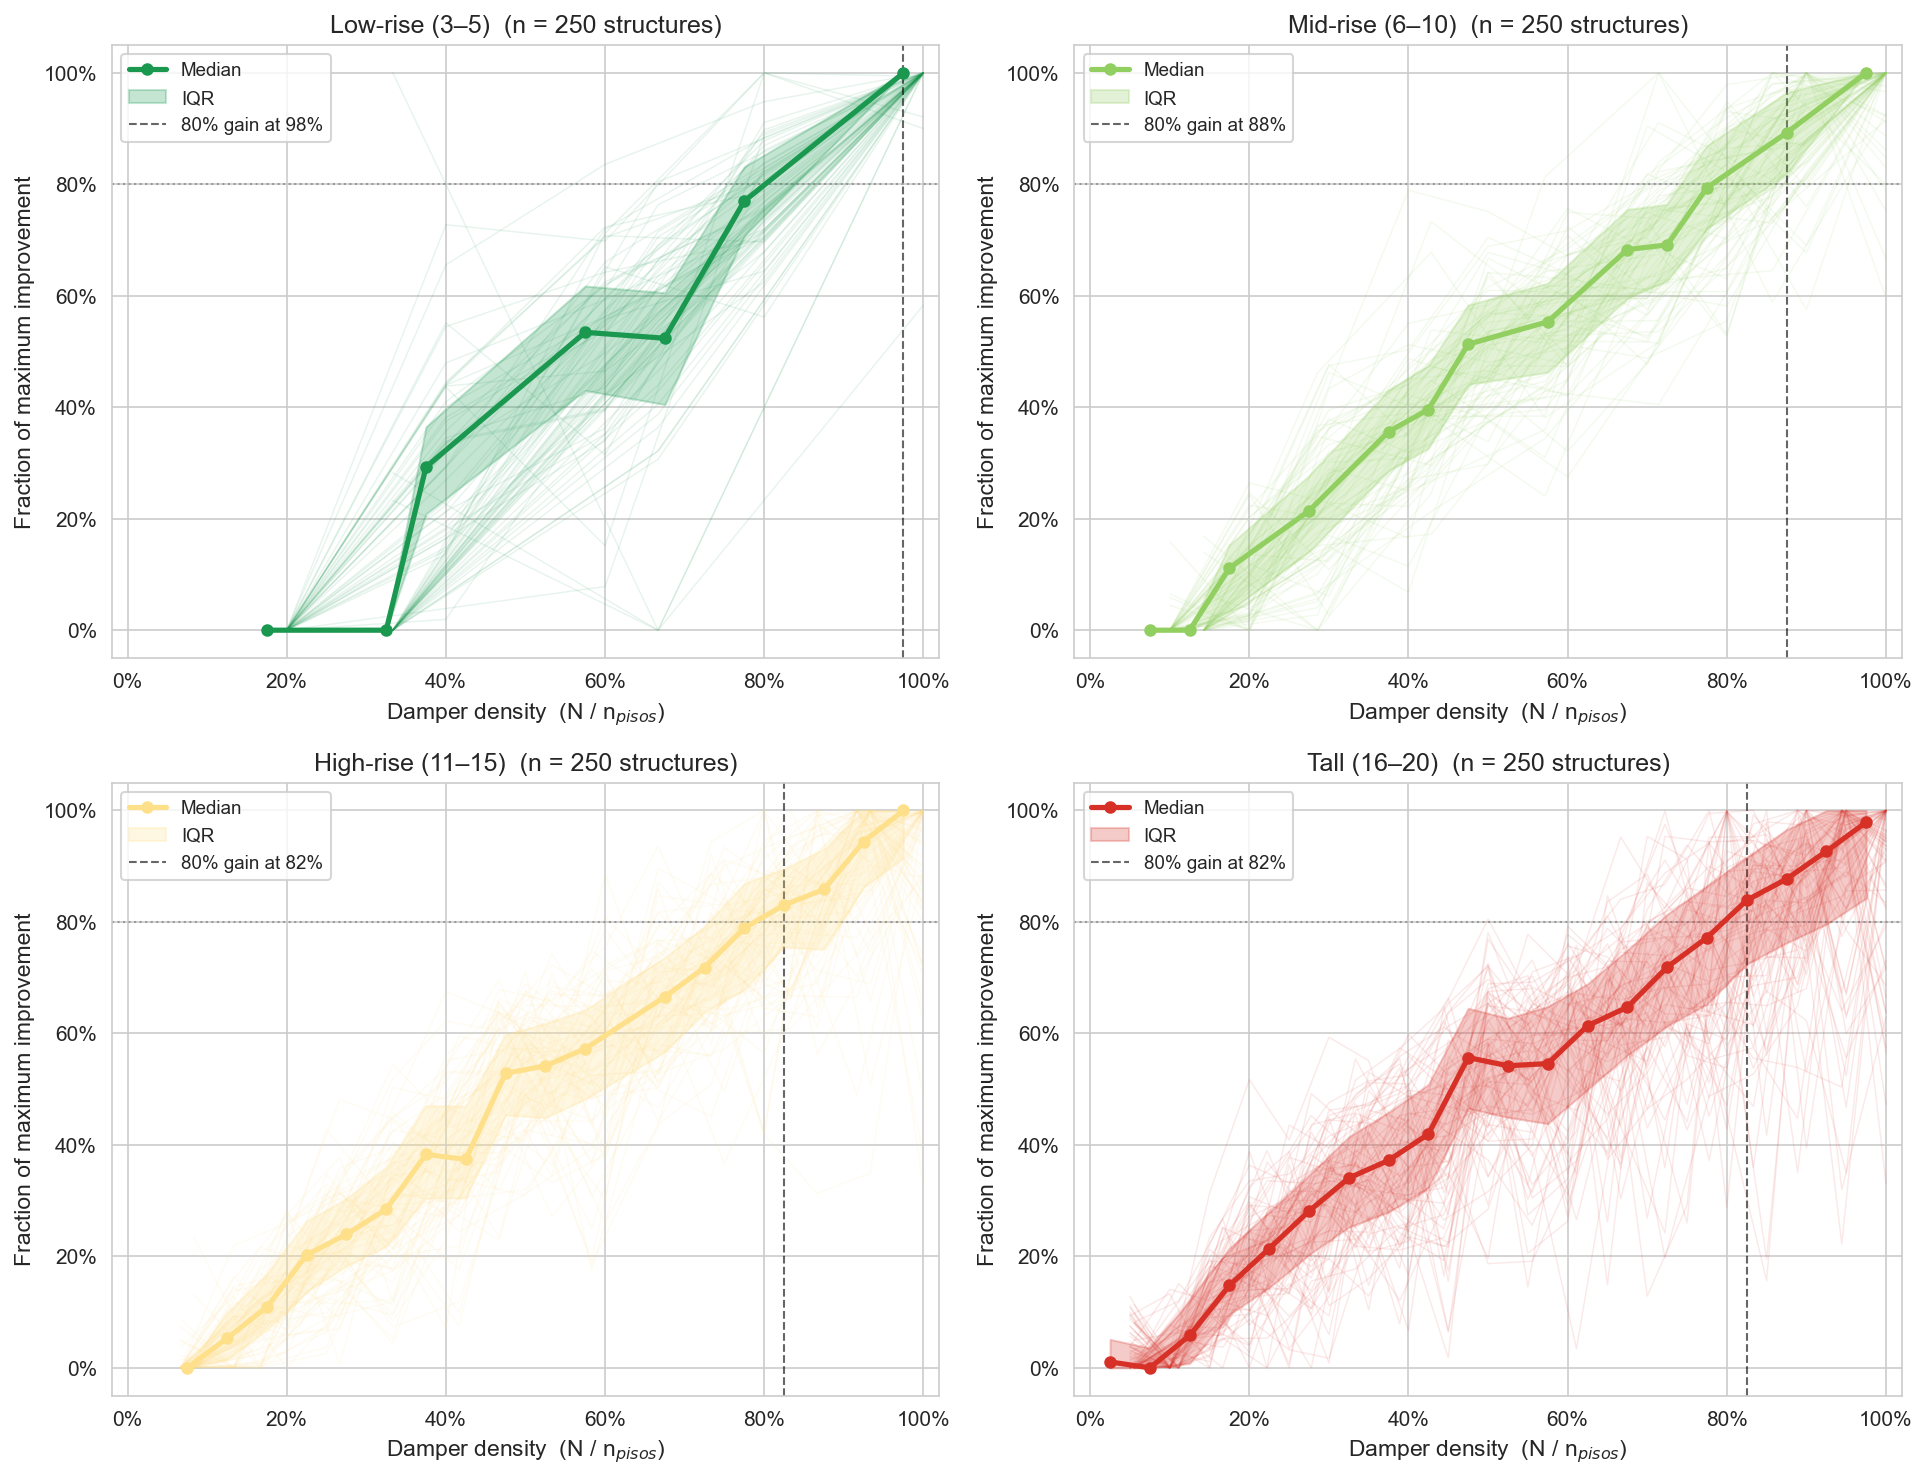
\includegraphics[width=\linewidth]{figs/F6_within_structure_curves.png}
\caption{Within-structure diminishing returns curves by height group. Each thin line represents an
individual structure; thick line is group median $\pm$ IQR. Vertical dashed line: density at which
80\% of maximum gain is achieved.}
\label{fig:curvas_internas}
\end{figure}

\subsection{Interaction between Damper Quantity and Frictional Moment}
\label{sec:results:interaccion}

\Cref{fig:mapa_calor} presents a two-dimensional heatmap of median $CR_2$ as a function of binned
$\nd$ and binned $\Mf$, stratified by three height groups (\cref{fig:mapa_calor}). Stratified analysis
reveals differentiated patterns that the global map does not capture.

In all three groups, low density combined with $\Mf \leq 100$\KM produces the highest $CR_2$ values (worst
performance), confirming that both variables act as necessary minimum constraints. However, the relative
weight of each variable varies with building height. In low-rise frames (3--5 stories) both $\nd$ and $\Mf$
contribute comparably: increasing $\nd$ from 1--2 to 3--4 with $\Mf \in [200,\,300]$\KM reduces $CR_2$ from
1.46 to 1.12, and raising $\Mf$ from 100 to 300\KM at fixed $\nd$ produces similar reductions, indicating
effective substitution between quantity and capacity. In mid-rise and high-rise frames (6--20 stories) $\nd$
dominates with increasing clarity: at any $\nd$ level, increasing $\Mf$ continues yielding improvements
($\Delta CR_2 \approx 0.37$--$0.46$ over the full $\Mf$ range), but the effect of adding devices
systematically exceeds that of increasing per-device capacity. Across no group is insensitivity to $\Mf$
observed at high coverage: even with $\nd \geq 11$, the difference between $\Mf < 100$\KM and $\Mf > 400$\KM
is 0.46 $CR_2$ units for mid-rise frames and 0.37 for tall frames.

The optimal configurations identified by the ML model for the 1,000 structures concentrate in
$\Mf \in [300,\,460]$\KM (median 400\KM, IQR~[269,\,456]\KM) with coverage fractions predominantly at or
near unity ($\tilde{\eta}_{0.50} = 1.0$).

\begin{figure}[htbp]
\centering
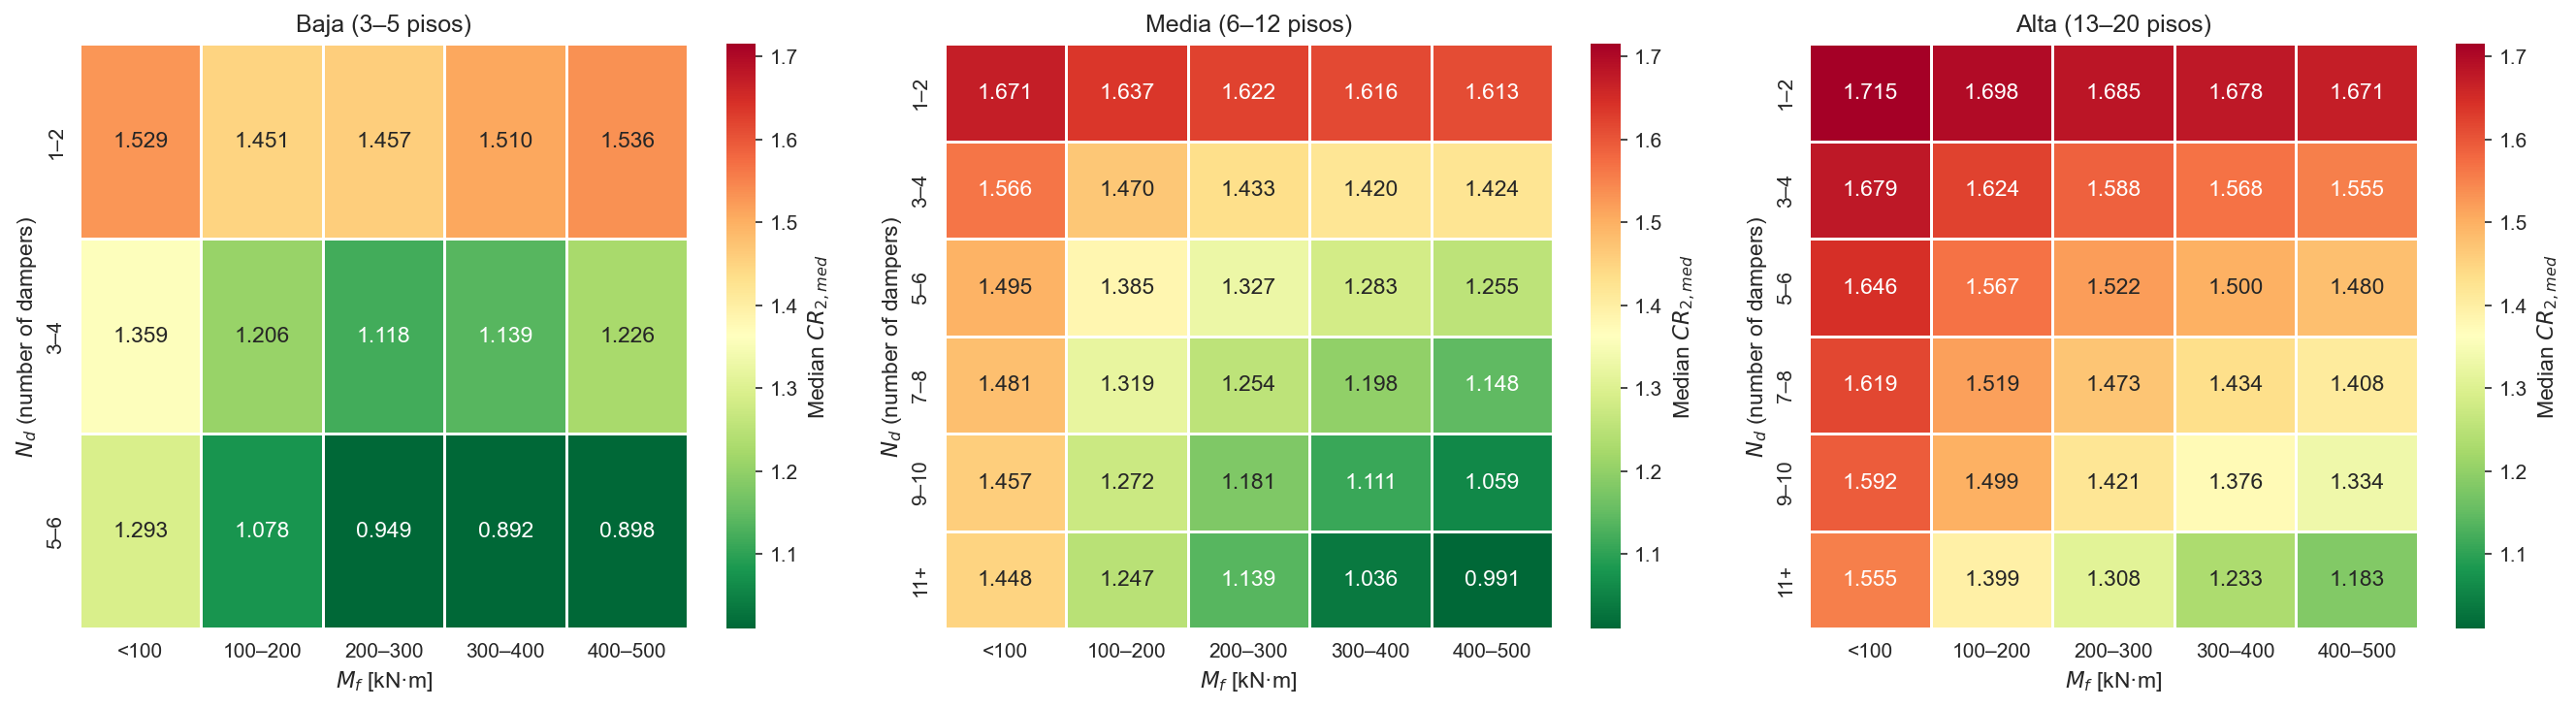
\includegraphics[width=\linewidth]{figs/F7_interaction_heatmap.png}
\caption{Left: median $CR_2$ as a function of $\nd$ bins and $\Mf$ bins (kN$\cdot$m), averaged
across all structures and records. Right: optimal $\nd$ vs.\ $\Mf$ for best configuration of each
structure (color: achieved $\CR{med}$).}
\label{fig:mapa_calor}
\end{figure}

\subsection{Design Convergence across Seismic Scenarios}
\label{sec:results:convergencia}

\Cref{fig:convergencia} examines whether a single optimal RFD design is robust across the three
seismic scenarios. For each of the 1,000 structures, optimal $\nd$ predicted under each target variable
was compared. Distribution of recommended $\nd$ is consistent across scenarios: median and P10 scenarios
produce nearly identical recommendations in most structures. The P90 scenario tends to recommend slightly
higher $\nd$ for taller buildings, but absolute discrepancy $|\nd^{\mathrm{P90}} - \nd^{\mathrm{med}}|$
remains below 2 for over 80\% of structures. This implies that a design optimized for the median scenario
provides near-optimal protection across all seismic variability captured by the eight-record ensemble.

\begin{figure}[htbp]
\centering
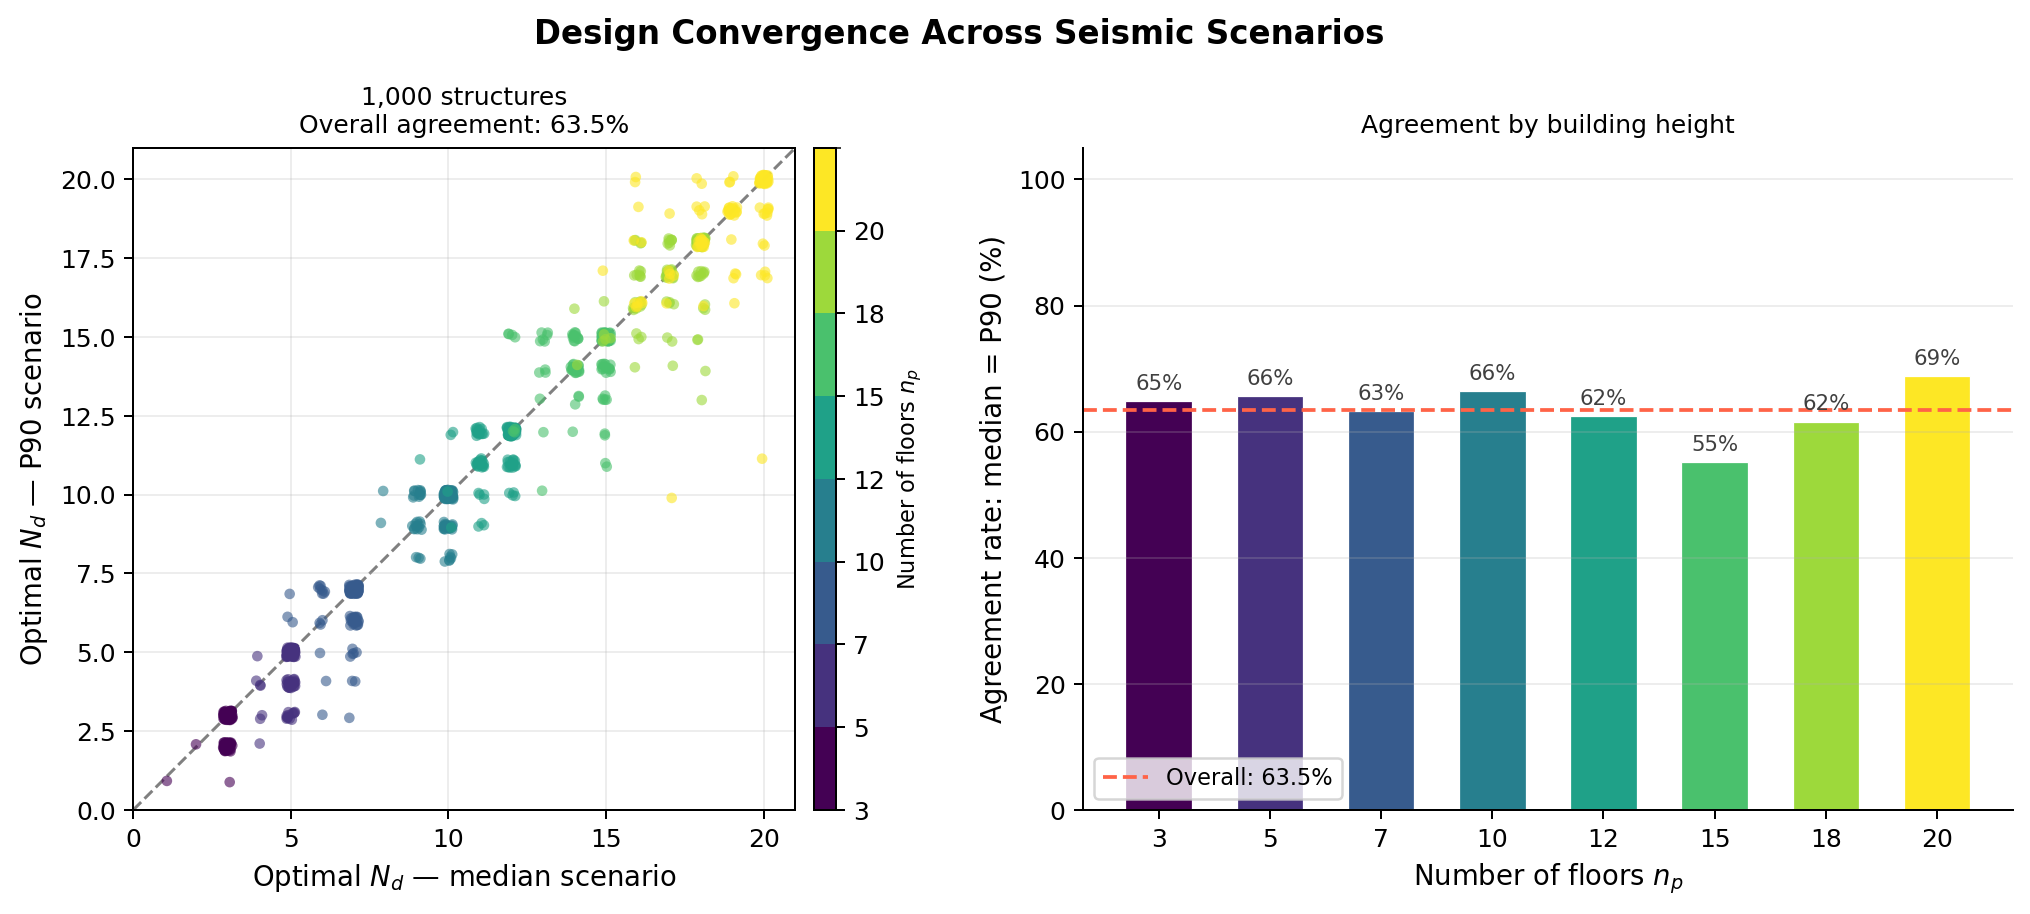
\includegraphics[width=\linewidth]{figs/F8_convergence_extended.png}
\caption{Left: distribution of recommended $\nd$ by seismic scenario across the 1,000 structures.
Right: agreement rate and mean absolute discrepancy $|\nd^{\mathrm{P90}} - \nd^{\mathrm{med}}|$
by building height $\np$.}
\label{fig:convergencia}
\end{figure}

%%═══════════════════════════════════════════════════════════════════════════
\section{Discussion}
\label{sec:discussion}
%%═══════════════════════════════════════════════════════════════════════════

\subsection{Density as Governing Design Parameter}

Coverage density $\etad$ emerges as the dominant predictor of $CR_2$ ($r = -0.73$), and its dominance
is robust: stochastic dominance analysis confirms this hierarchy holds across the eight seismic records
independent of other design variables (Section~\ref{sec:results:decreciente}). Based on the 80\% maximum
gain threshold analysis, the following design recommendation is derived: $\etad \geq 0.85$ for mid-rise
and tall frames (6--20 stories), and $\etad \geq 0.90$ for low-rise frames (3--5 stories), where
proportional impact of each additional device is greater.

\subsection{Interaction between Frictional Moment and Coverage}

The heat map analysis (\cref{fig:mapa_calor}) reveals a substitution relationship between $\nd$
and $\Mf$ at intermediate coverage levels: doubling $\Mf$ at fixed count produces $CR_2$ reductions
similar to increasing $\nd$ by two stories. This interaction is not captured by marginal correlation
analysis and motivates the use of ensemble ML models that explicitly represent nonlinear feature
interactions. At high coverage ($\etad \geq 0.75$), performance becomes relatively insensitive to the
specific $\Mf$ value within the [200,\,500]\KM range, and the ML-identified optimal range,
$\Mf \in [300,\,460]$\KM, is consistent with the optimal $\Mf = 257.9$\,kips$\cdot$in $\approx 290$\KM
reported by \citet{Jarrahi2020jbe} for a single-story MRSF under higher-intensity excitation.

\subsection{Robustness across Scenarios}

The high level of agreement between design recommendations of the median and P90 scenarios (\cref{fig:convergencia})
implies that separate optimization problems need not be solved for different seismic hazard levels when the
objective is to identify optimal $\nd$. The multi-record approach directly addresses the limitation of
single-record optimization studies \citep{Jarrahi2020jbe,Jarrahi2020sdee}, capturing record-to-record
variability in P10, median, and P90 statistics, making ML recommendations inherently robust to uncertainty
in accelerogram selection.

\subsection{Limitations}

The following limitations should be acknowledged. (i)~Structural models are idealized elastic shear frames;
explicit frame--RFD nonlinear interaction is not captured. (ii)~The eight accelerograms, though seismically
diverse, may not represent all relevant tectonic settings. (iii)~Model validation relies only on
cross-validation; an independent test set would provide more rigorous generalization assessment. (iv)~A
uniform $\Mf$ value per structure is assumed; story-specific $\Mf$ distributions may be preferable in
practice. (v)~No cost function is incorporated, so economic optimization of coverage fraction is not
addressed.

%%═══════════════════════════════════════════════════════════════════════════
\section{Conclusions}
\label{sec:conclusions}
%%═══════════════════════════════════════════════════════════════════════════

The following main conclusions are derived from analysis of $\approx$434,000 nonlinear time-history
simulations across 1,000 diverse structural configurations and eight real seismic records:

\begin{enumerate}

\item \textbf{Accuracy of ML surrogate model.}
XGBoost and Random Forest achieved $\Rsq$ of 0.92--0.93 for $\CR{med}$ and $\CR{P10}$, and 0.84 for
$\CR{P90}$. Ensemble models reduced prediction error by approximately 49\% relative to linear baselines,
quantifying the nonlinear structure of the design--performance relationship.

\item \textbf{Damper density is the primary design variable.}
Coverage fraction $\etad = \nd/\np$ is the most influential predictor ($r = -0.73$), substantially
outperforming absolute damper count ($r = -0.45$). Design guidelines for RFDs should be expressed in
terms of $\etad$, not $\nd$.

\item \textbf{Diminishing returns threshold: $\etad \approx 0.85$.}
Within-structure analysis reveals that 80\% of maximum $CR_2$ reduction is achieved at $\etad \approx 0.85$
for mid-rise and tall frames (6--20~stories) and at $\etad \approx 0.95$ for low-rise frames (3--5~stories).
These thresholds provide practical cost-effectiveness criteria for RFD deployment.

\item \textbf{Optimal range of frictional moment.}
Across the 1,000 analyzed structures, optimal $\Mf$ identified by ML concentrates in [300,\,460]\KM
(median 400\KM). For $\etad \geq 0.75$, $CR_2$ is relatively insensitive to the specific $\Mf$ value
within [200,\,500]\KM, making coverage fraction the most critical design parameter.

\item \textbf{Robustness across scenarios.}
Optimal $\nd$ recommended by median and P90 scenarios differs by fewer than 2 stories in 80\% of analyzed
structures, confirming that a design optimized for the median scenario provides near-optimal protection
across all seismic variability in the eight-record ensemble.

\item \textbf{Future work.}
Extensions should incorporate inelastic frame behavior, story-specific $\Mf$ distributions, installation
cost constraints, and broader seismic record suites representing different tectonic environments.
Experimental validation for multi-story configurations and integration of trained models into an
interactive design tool represent immediate research directions.

\end{enumerate}

%%═══════════════════════════════════════════════════════════════════════════
\bibliographystyle{elsarticle-harv}
\bibliography{references}

\end{document}
